%%%%%%%%%%%%%%%%%%%%%%%%%%%%%%%%%%%%%%%%%%%%%%%%%%%%%%%%%%%%%%%%%%%%%%%%%%%%%%%
%% Template de Relatório Parcial baseado nas normas da ABNT voltado 
%% para alunos da UEFS, baseado no modelo de TCC
%% Versão 1.3
%% Desenvolvimento: Danilo de Oliveira Gonçalves
%% Adaptação final: João Carlos Nunes Bittencourt
%% Data: 31/03/2011
%% Atualização: 11/08/2011
%
% TODO: Ajustar o espaçamento do cabeçalho do Apêndice e do Anexo.
%%%%%%%%%%%%%%%%%%%%%%%%%%%%%%%%%%%%%%%%%%%%%%%%%%%%%%%%%%%%%%%%%%%%%%%%%%%%%%%
\documentclass[unknownkeysallowed]{abnt-uem} % Classe de formatação
\usepackage[alf,abnt-emphasize=bf]{abnt-alf}
\usepackage[utf8]{inputenc}
\usepackage[brazil]{babel}
\usepackage[pdftex]{graphicx}
\usepackage{subfigure}
\usepackage{caption}
\usepackage[font=small,labelfont=bf]{caption}
\usepackage{longtable}
\usepackage{float} % para as figuras ficarem onde foram colocadas no latex - deve colcoar na figura [H]
\usepackage{enumerate}
\usepackage{pbox}
\usepackage{multirow}% http://ctan.org/pkg/multirow
\usepackage{hhline}% http://ctan.org/pkg/hhline
\usepackage{tikz}
\def\checkmark{\tikz\fill[scale=0.5](0,.35) -- (.25,0) -- (1,.7) -- (.25,.15) -- cycle;}
\graphicspath{{./figuras/}} % Diretório padrão de figuras.

%%%%%%%%%%%%%%%%%%%%%%%%%%%%%%%%%%%%%%%%%%%%%%%%%%%%%%%%%%%%%%%%%%%%%%%%%%%%%%%
% Este arquivo faz parte do template de Relatório Parcial baseado nas normas da ABNT 
%  voltado para alunos da UEFS
% Desenvolvimento: Danilo de Oliveira Gonçalves
% Adaptação final: João Carlos Nunes Bittencourt
% Data: 31/03/2011
% Atualização: 30/11/2011
% Descrição do arquivo:
%   Esse arquivo apresenta as definições de constantes que formarão a capa e 
%   a folha de rosto. Siga as instruções e modifique de acordo com o que
%   lhe foi orientado.
%%%%%%%%%%%%%%%%%%%%%%%%%%%%%%%%%%%%%%%%%%%%%%%%%%%%%%%%%%%%%%%%%%%%%%%%%%%%%%%

% ---------- Preambulo ----------
\instituicao{Universidade Estadual de Maringá} % nome da instituicao
\departamento{Departamento de Informática}
\graduacao{Informática} % nome do curso
\curso{Informática}

\documento{Trabalho de Conclusão de Curso} % tipo de documento
\titulacao{Bacharel} % [Bacharel]

%\titulo{Redes de Computadores} % titulo do trabalho em portugues
\subtitulo{Uso de informações de contexto para controle de acesso em provedores de conteúdo} % caso necessário um sub-título, utilize este campo
%\title{Title in English} % titulo do trabalho em ingles

\autor{Anderson de Souza Zanichelli} % autor do trabalho
\cita{ZANICHELLI, Anderson de Souza Zanichelli} % sobrenome (maiusculas), nome do autor do trabalho

\comentario{\UEFSdocumentodata\ apresentado ao \UEFSdepartamentodata\ como requisito parcial para obtenção do grau de \UEFStitulacaodata\ em \UEFScursodata\ da \ABNTinstituicaodata.}

%\orientador{Profa. Dra. Luciana Andréia Fondazzi Martimiano} % nome do orientador do trabalho
\orientador[Orientadora:]{Profa. Dra. Luciana Andréia Fondazzi Martimiano} % <- no caso de orientadora, usar esta sintaxe
%\coorientador{Nome do Co-orientador} % nome do co-orientador do trabalho, caso exista
%\coorientador[Co-orientadora:]{Nome da Co-orientadora} % <- no caso de co-orientadora, usar esta sintaxe

\local{Maringá} % cidade
\data{2016} % ano



 % Elementos da capa
\begin{document}
    \pagestyle{empty}
    \DeclareGraphicsExtensions{.jpg,.pdf,.mps,.png,.bmp,.eps}
    
\vspace{5cm}
Carta de Encaminhamento da Monografia

\vspace{2cm}
\hfill Maringá, 15 de Fevereiro de 2016.

\vspace{3cm}
À Coordenação de Trabalho de Graduação

Departamento de Informática

Centro de Tecnologia

Universidade Estadual de Maringá

\vspace{3cm}
Encaminhamos, em anexo, a monografia intitulada "Uso de informações de contexto para controle de acesso em provedores de conteúdo"

\begin{center}
\vspace{3cm}

\makebox[3in]{\hrulefill}\\
Anderson de Souza Zanichelli

(aluno)

\vspace{3cm}
\makebox[3in]{\hrulefill}\\
Professora Dra. Luciana Andréia Fondazzi Martimiano

(orientadora)
\end{center}
    \capa % geração automática da capa
    \folhaderosto % geração automática da folha de rosto
    %%%%%%%%%%%%%%%%%%%%%%%%%%%%%%%%%%%%%%%%%%%%%%%%%%%%%%%%%%%%%%%%%%%%%%%%%%%%%%%
%% Este arquivo faz parte do template de TCC baseado nas normas da ABNT 
%%  voltado para alunos da UEFS
%% Desenvolvimento: Danilo de Oliveira Gonçalves
%% Adaptação final: João Carlos Nunes Bittencourt
%% Data: 31/03/2011
%%%%%%%%%%%%%%%%%%%%%%%%%%%%%%%%%%%%%%%%%%%%%%%%%%%%%%%%%%%%%%%%%%%%%%%%%%%%%%%


% dedicatória (opcional)
\begin{dedicatoria}
À minha esposa Maria Ester e minha filha Anna Laura que tiveram que lidar com as minhas ausências.
\end{dedicatoria}

%\vfill

%\begin{flushright}
%\hfill \textit{Dedico esta monografia a minha família,\\pelo apoio fornecido e aos meus amigos.\\}
%\end{flushright}

%\vspace*{1cm}

%\clearpage 

    %%%%%%%%%%%%%%%%%%%%%%%%%%%%%%%%%%%%%%%%%%%%%%%%%%%%%%%%%%%%%%%%%%%%%%%%%%%%%%%
%% Este arquivo faz parte do template de TCC baseado nas normas da ABNT 
%%  voltado para alunos da UEFS
%% Desenvolvimento: Danilo de Oliveira Gonçalves
%% Adaptação final: João Carlos Nunes Bittencourt
%% Data: 31/03/2011
%%%%%%%%%%%%%%%%%%%%%%%%%%%%%%%%%%%%%%%%%%%%%%%%%%%%%%%%%%%%%%%%%%%%%%%%%%%%%%%

% agradecimentos (opcional)
\begin{agradecimentos}
Agradeço à minha orientadora Professora Dra. Luciana Andréia Fondazzi Martimiano que sempre foi compreensiva, sempre ofereceu ideias enriquecedoras e que confiou no meu trabalho.

Agradeço à minha esposa Maria Ester que me motivou e que cuidou da nossa filha com dedicação enquanto eu precisava voltar minha atenção aos estudos.

Agradeço à minha mãe que me ensinou a tratar os estudos como algo importante.

Agradeço aos professores do Departamento de Informática da Universidade Estadual de Maringá pelo trabalho que realizam.

Agradeço aos meus amigos que foram companheiros e que ofereceram o seu tempo para me ensinar coisas que eu precisava aprender. 
\end{agradecimentos}

    \begin{resumo}
Com o uso das redes sem fios, que disponibilizam Internet nos dispositivos móveis, a quantidade de serviços e conteúdos oferecidos aos usuários é imensa e como cada provedor de conteúdo pode apresentar atributos relacionados aos serviços oferecidos, como por exemplo: número de clientes conectados, tempo de resposta, custo e qualidade do serviço, os valores desses atributos podem ser modificados dependendo da situação do provedor. Dessa forma, o conjunto de atributos pode ser relevante para o usuário no momento da escolha do provedor de conteúdo que atenderá suas expectativas de forma satisfatória, caso não esteja sendo atendido, o usuário irá procurar outro serviço semelhante que lhe atenda da forma desejada. Assim, neste trabalho foram implementadas duas aplicações, uma aplicação servidora que realiza a escolha do serviço que melhor atende às configurações dos atributos definidas pelo usuário e que também realiza as autenticações nos serviços de forma transparente e uma aplicação para dispositivos móveis onde o usuário realiza a configuração dos atributos de acordo com suas preferências e que também é consumidora dos serviços escolhidos de forma automatizada pela aplicação servidora.
\end{resumo}	

    \begin{abstract}
With the use of wireless networks that deliver Internet on mobile devices, the number of services and content offered to users is immense and as each content provider that the user accesses may have attributes related to the services offered, such as: number of connected clients, response time, cost and quality of service, the values of these attributes can be modified depending on the provider's situation. Thus, the set of attributes may be relevant to the user when choosing the content provider that will meet your expectations in a satisfactory manner, if not being met, the user will look for another similar service that suits the way the user want. In this work were implemented two applications, a server application which choose the service that best suits the attributes defined by the user and also performs authentications in a transparent manner and an application for mobile devices where the user performs configuration of attributes according to his/her preferences and is also consuming the services chosen automated way by the server application.
\end{abstract}

    \listadefiguras % geracao automatica da lista de figuras
    \listadetabelas % geracao automatica da lista de tabelas
    %\listadesimbolos % geracao automatica da lista de símbolos
    \listadesiglas % % geracao automatica da lista de siglas
    % sumario
    \sumario % geracao automatica do sumario
    %---------- Primeiro Capitulo ----------
\chapter{Introdução}\label{cha:introducao}

A evolução tecnológica, presente nos dias de hoje, possibilitou o desenvolvimento de dispositivos móveis que não são mais usados somente para a comunicação, mas para a execução de diversas aplicações que oferecem funcionalidades com alta qualidade de serviço, para as quais, há alguns anos atrás seriam necessários diversos equipamentos dedicados, como no exemplo da Figura \ref{fig:convergencia} onde podemos perceber a convergência de algumas funcionalidades desses aparelhos para os dispositivos móveis: um aparelho de som, aparelho dedicado para o uso de \sigla{GPS}{Global Positioning System} (\textit{Global Positioning System}), câmera de alta resolução para tirar fotos e realizar a gravação de áudio e vídeo, computador para a comunicação através de redes \sigla{Wi-Fi}{Wireless Fidelity} (\textit{Wireless Fidelity}) e também o uso de \textit{video-games}.

\begin{figure}[!htb]
	\centering
	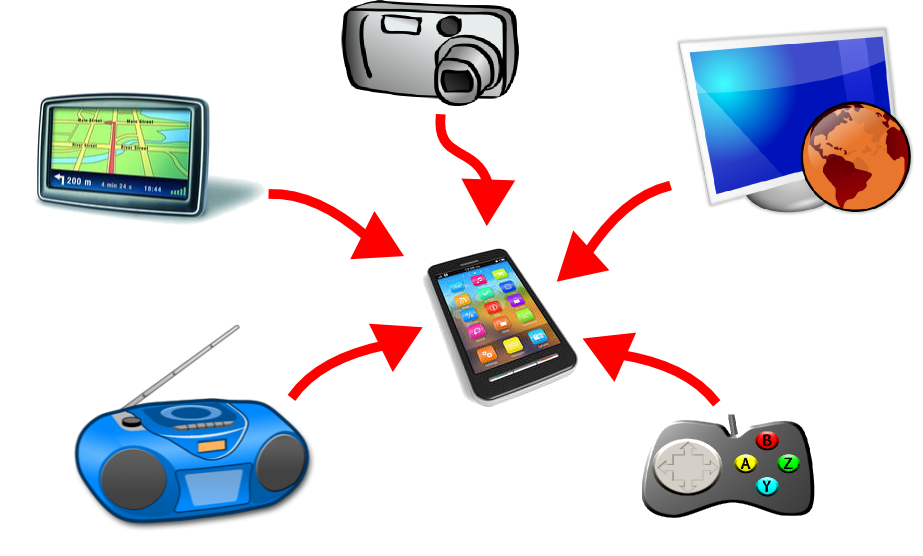
\includegraphics[width=0.5\textwidth]{convergencia.png} % <- formatos PNG, JPG e PDF
	\small
	\caption[Convergência de diversos equipamentos para um dispositivo móvel]{Convergência de diversos equipamentos para um dispositivo móvel}
	\label{fig:convergencia}
\end{figure}

Com o uso das redes sem fios, que disponibilizam o uso da Internet nos dispositivos móveis, a quantidade de serviços e conteúdos oferecidos aos usuários é imensa. Podem ser utilizados serviços como: correio eletrônico, navegação em sites, troca de mensagens instantâneas, download e upload de arquivos, conexão a bancos de dados, o uso de streaming de áudio e vídeo, e tudo o mais que a Internet possa oferecer.

Todos esses serviços e produtos que estão disponíveis na Internet se beneficiam da qualidade das redes de computadores, como por exemplo, uma boa largura de banda e equipamentos de última geração, mas também podem ser prejudicados por alguma deficiência ou problema que aconteça com a rede, como o defeito em algum roteador, o congestionamento na rede ou uma arquitetura mal dimensionada. Assim, cada um dos provedores de conteúdo que o usuário acessa pode apresentar atributos relacionados aos serviços oferecidos, como por exemplo: número de clientes conectados, tempo de resposta, custo da licença para usar o serviço e a qualidade do serviço prestada.

Os valores desses atributos podem ser modificados dependendo do contexto em que se encontra esse provedor. Dessa forma, esse conjunto de atributos pode ser relevante para o usuário no momento da escolha do provedor de conteúdo que atenderá as suas expectativas de forma satisfatória. Como essas informações podem ser alteradas, um serviço escolhido poderá não mais atender ao usuário de forma satisfatória, assim ele poderá procurar outro serviço semelhante que lhe atenda da forma desejada. Neste trabalho, essas informações são importantes para que seja feita a escolha do provedor de serviço de forma automatizada, elas determinam qual é o provedor que o usuário escolheria.

Este trabalho tem como base o trabalho realizado na dissertação de mestrado em Ciência da Computação de \cite{praca12}, onde foi descrito um modelo de autenticação baseado em informações de contexto, denominado HandProv, no qual o usuário efetua handover (troca de conexão de um ponto de acesso para outro sem perda ou interrupção dos serviços) de provedores de serviço de forma transparente. As trocas de provedores aconteciam baseando-se nos valores de alguns atributos, onde o gerente de aplicações escolhia o provedor que melhor atendesse ao usuário. 

\section{Motivação}
O grande salto na quantidade de dispositivos móveis utilizados pela população em geral, fez com que aparecessem novas necessidades de software. Alguns desses sistemas têm como objetivo a facilitação de resolução de tarefas do cotidiano do usuário.
A disseminação do uso das redes sem fio, Wi-Fi e 3G, que possibilitam aos usuários estarem conectados à Internet, com uma boa largura de banda, faz com que os usuários passem uma parte considerável de seu tempo utilizando serviços e recursos disponibilizados pela rede.
Devido a essa grande quantidade de serviços disponíveis e muitos deles oferecendo o mesmo tipo de conteúdo o usuário tem a opção de escolher o que atenda-o da melhor maneira.

\section{Objetivos e Contribuições}
Este trabalho teve como objetivo a implementação de duas aplicações, uma aplicação para dispositivos móveis onde o usuário configura os seus requisitos para cada provedor de serviço e que também apresenta os serviços ao usuário e uma aplicação servidora que realiza a escolha de qual serviço atende aos requisitos do usuário e que realiza as autenticações necessárias nos serviços de forma transparente.

Através dos estudos realizados sobre as tecnologias utilizadas e das implementações dos sistemas, este trabalho ficará disponível à comunidade acadêmica como um exemplo de uma aplicação desenvolvida para dispositivos móveis que utiliza novas tecnologias, como por exemplo um banco de dados NoSQL\footnote{Sistemas de bancos de dados que utilizam formas de armazenar e devolver dados diferente dos que utilizam tabelas relacionais} e o desenvolvimento utilizando ferramentas disponibilizadas na nuvem.

A contribuição que este trabalho faz em relação ao trabalho de \cite{praca12} é a apresentação de um modelo onde são os provedores de serviço que determinam quais são seus atributos e o usuário apenas configura os valores que ele considera relevantes a ele, e a implementação de uma estrutura na aplicação do dispositivo móvel que permite a renderização de formulários dinâmicos, que pode sofrer alterações no seu desenho de acordo com as alterações dos atributos dos provedores sem a necessidade de alterações no código fonte da aplicação.

\section{Organização do trabalho}
Neste trabalho o termo 'Dispositivos Móveis' será utilizado para representar o termo em inglês Smartphones, que categoriza uma linha de aparelhos celulares com sistemas operacionais multitarefas.

Este trabalho está organizado da seguinte maneira. O Capítulo \ref{cha:introducao} apresenta o cenário no qual o trabalho se encaixa, a motivação e os objetivos desse trabalho. O Capítulo \ref{cha:fundamentacao} apresenta os principais conceitos sobre autenticação em sistemas computacionais. O Capítulo \ref{cha:visaogeral} apresenta algumas das principais tecnologias sobre dispositivos móveis presentes no mercado atualmente. O Capítulo \ref{cha:ferramentas} apresenta algumas das tecnologias mais conhecidas para o desenvolvimento de aplicativos móveis. O Capítulo \ref{cha:desenvolvimento} apresenta os sistemas que foram implementados e como eles funcionam. O Capítulo \ref{cha:conclusao} finaliza o trabalho de conclusão de curso com as contribuições e trabalhos futuros.
    %---------- Segundo Capitulo ----------
\chapter{Fundamentação Teórica}\label{cha:fundamentacao}
\section{Autenticação}
Em sistemas computacionais em que a identificação e autenticação do usuário são premissas na segurança de transações e processos, é interessante manter mecanismos que ofereçam aos usuários, meios confiáveis no estabelecimento dessas conexões. Segundo \cite{tanenbaum2011computer} esse era um problema inexistente no início das comunicações pelas redes de computadores.
\begin{citacao}
Durante as primeiras décadas de sua existência, as redes de computadores foram usadas principalmente por pesquisadores universitários, com a finalidade de enviar mensagens de correio eletrônico, e também por funcionários de empresas, para compartilhar impressoras. Sob essas condições, a segurança nunca precisou de maiores cuidados. Porém, como milhões de cidadãos comuns atualmente estão usando as redes para executar operações bancárias, fazer compras e arquivar sua devolução de impostos, a segurança das redes está despontando no horizonte como um problema potencial.\cite{tanenbaum2011computer}
\end{citacao}
Frequentemente para utilizar algum recurso computacional é utilizada alguma das três técnicas de autenticação de usuários:

\begin{enumerate}[(a)]
	\item Algo que o usuário sabe – uma senha, a resposta para alguma pergunta ou reconhecimento de algum padrão;
	\item Algo que o usuário tem – um cartão magnético, um crachá ou um \textit{token} de segurança;
	\item Como o usuário é – baseado em características biométricas.
\end{enumerate}

As técnicas (a) e (b) podem ser passíveis de fraude, tendo em vista que alguém possuindo tais informações/objetos pode facilmente conseguir acesso ao sistema como se fosse o verdadeiro usuário. Além disso, esses fatores necessitam da interação direta do usuário, isto é, o usuário deve informar estes dados para realizar a autenticação, geralmente via dispositivos de entrada comuns, como microfone, teclado ou tela, como no exemplo da Figura \ref{fig:trace}, onde é necessário o reconhecimento de um determinado padrão.
\vspace{3cm}

\begin{figure}[!htb]
	\centering
	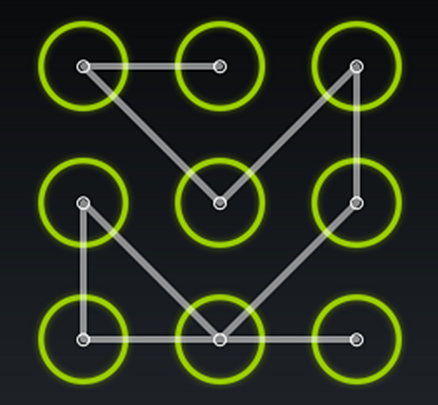
\includegraphics[width=0.2\textwidth]{trace.png} % <- formatos PNG, JPG e PDF
	\small
	\caption[Uso de senha por reconhecimento de padrão]{Uso de senha por reconhecimento de padrão nos \textit{smartphones} Android}
	\label{fig:trace}
\end{figure}

\subsection{O uso de senhas}
Mesmo a autenticação através do uso de senhas ser o alvo de várias formas de ataque, como podemos perceber na citação abaixo de um trecho da cartilha de segurança do CERT \cite{Cert2016}, ela é uma das mais empregadas como meio de assegurar a privacidade de sistemas.
\begin{citacao}
Algumas das formas como a sua senha pode ser descoberta são:
	\begin{enumerate}
		\item Ao ser usada em computadores infectados. Muitos códigos maliciosos, ao infectar um computador, armazenam as teclas digitadas (inclusive senhas), espionam o teclado pela webcam (caso você possua uma e ela esteja apontada para o teclado) e gravam a posição da tela onde o mouse foi clicado;
		\item Ao ser usada em sites falsos. Ao digitar a sua senha em um site falso, achando que está no site verdadeiro, um atacante pode armazená-la e, posteriormente, usá-la para acessar o site verdadeiro e realizar operações em seu nome;
		\item Ao ser capturada enquanto trafega na rede, sem estar criptografada;
		\item Com o uso de técnicas de engenharia social, como forma a persuadi-lo a entregá-la voluntariamente;
		\item Pela observação da movimentação dos seus dedos no teclado ou dos cliques do mouse em teclados virtuais.
	\end{enumerate}
\end{citacao}

Na tentativa de melhorar a segurança de seus sistemas e melhorar a eficiência no uso de senhas muitas organizações adotam políticas de segurança que impõem regras no uso das senhas, além disso, criam mecanismos para que as senhas tenham um determinado formato, utilizam algum algoritmo de criptografia e as senhas podem expirar em um determinado tempo.

A \sigla{NBR ISO/IEC 27001}{NBR ISO/IEC 27001 - Tecnologia da informação - Técnicas de segurança - Sistemas de gestão de segurança da informação - Requisitos} (NBR ISO/IEC 27001 - Tecnologia da informação - Técnicas de segurança - Sistemas de gestão de segurança da informação - Requisitos) apresenta aos gestores de segurança da informação sugestões de controles que podem ser adotados nas organizações, como os da Tabela \ref{tab:ISO17}.

\begin{table}[!htb]
  	\centering
  	\footnotesize
	\caption[Objetivos de controle e controles na ABNT NBR ISO/IEC 27001]{Objetivos de controle e controles apresentados na ABNT NBR ISO/IEC 27001 \cite{nbr27001}}
	\begin{tabular}{|*3{c|}} \hline
		\multicolumn{3}{|c|}{A.11.2 Gerenciamento de acesso do usuário}\\ \hline
		A.11.2.1 & Registro de usuário & \vtop{\hbox{\strut Controle}\hbox{\strut Deve existir um procedimento formal de registro e}\hbox{\strut cancelamento de usuário para garantir e revogar }\hbox{\strut acessos em todos os sistemas de informação}\hbox{\strut e serviços.}} \\ \hline
		A.11.2.3 & \vtop{\hbox{\strut Gerenciamento de}\hbox{\strut senha do usuário}} & \vtop{\hbox{\strut Controle}\hbox{\strut A concessão de senhas deve ser controlada}\hbox{\strut por meio de um processo de gerenciamento formal.}} \\ \hline
	\end{tabular}
	\label{tab:ISO17}
\end{table}

\subsection{O uso de \normalfont\itshape tokens}
O uso de senhas pode não ser seguro o suficiente para garantir a autenticidade e confidencialidade do usuário em alguns tipos de sistemas, como por exemplo o acesso a contas bancárias ou o acesso ao \sigla{SGBD}{Sistema de gerenciamento de banco de dados} (Sistema de gerenciamento de banco de dados) de uma aplicação crítica. Nesses sistemas é comum o uso de \textit{tokens}.

\textit{Tokens} são pequenos dispositivos, do tamanho de um chaveiro, como o exemplo apresentado na Figura \ref{fig:token}, cujo nome técnico é \textit{Token} \sigla{OTP}{One Time Password} (\textit{One Time Password}). Eles geram uma sequência numérica que será utilizada como uma senha mas por um pequeno espaço de tempo, por volta de 60 segundos, depois desse tempo essa sequência numérica perde a validade. Segundo a \cite{rfc2289} existem formas de ataques que podem capturar informações de identificação de um usuário e o uso de \textit{tokens} inutilizaria essas informações.

\begin{citacao}
Uma das formas de ataque em sistemas de computação em redes utilizam \textit{softwares} que escutam as conexões para obter informações de autenticação, tais como o \sigla{ID}{Identificação} (Identificação) e senha de usuários. Uma vez que esta informação é capturada, pode ser utilizado mais tarde para obter acesso ao sistema. Sistemas de senha de uso único são projetados para combater este tipo de ataque, chamado de "ataque de repetição".\cite{rfc2289}
\end{citacao}

\vspace{-3mm}
\begin{figure}[!htb]
	\centering
	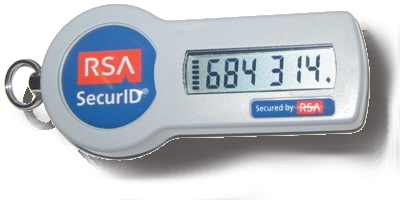
\includegraphics[width=0.3\textwidth]{token.png}
	\vspace{-3mm}
	\footnotesize
	\caption[Dispositivo gerador de \textit{tokens}]{Dispositivo gerador de \textit{tokens} Fonte: \cite{rationalcdn}}
	\label{fig:token}
\end{figure}

Além de dispositivos geradores de \textit{tokens}, como no exemplo da Figura \ref{fig:token} existem aplicativos com a mesma função, um exemplo é o \textit{Google Authenticator}, apresentado na Figura \ref{fig:tokenapp}. Nele são registrados os sistemas ao qual o usuário tem acesso, e quando necessário, o usuário utiliza a sequência numérica gerada pelo aplicativo.

\vspace{-3mm}
\begin{figure}[!htb]
	\centering
	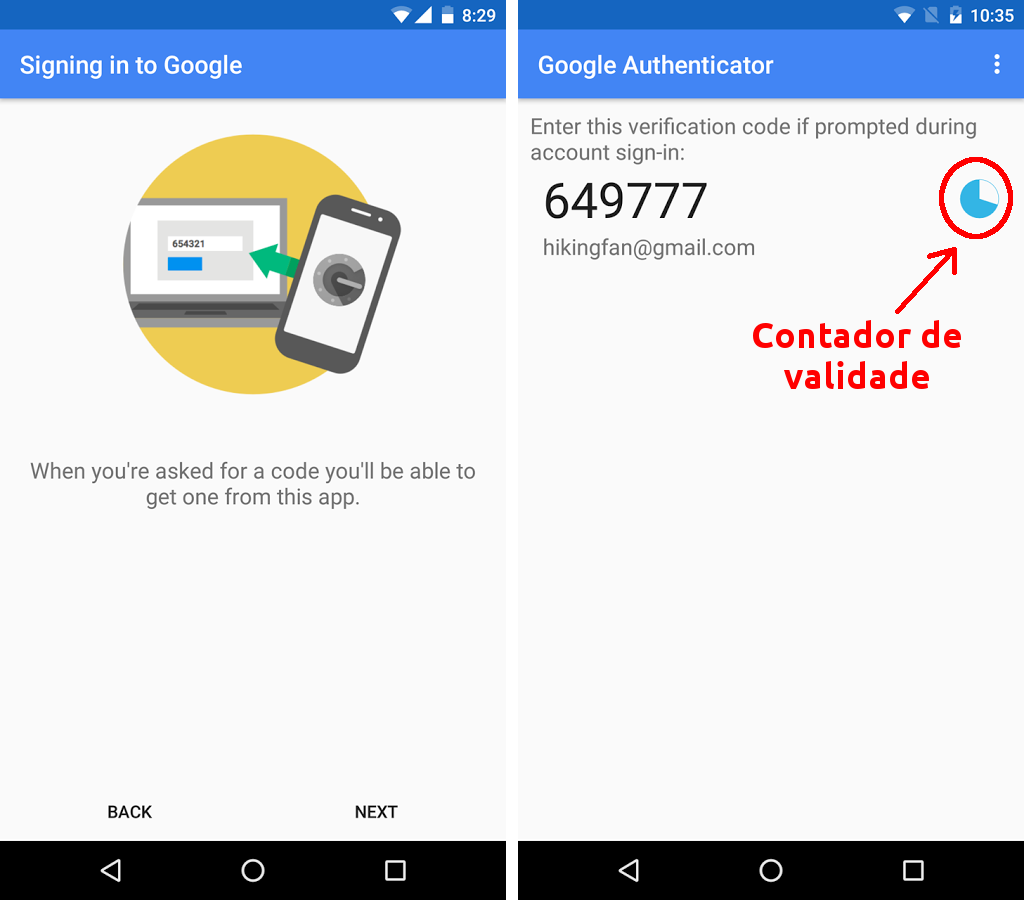
\includegraphics[width=0.5\textwidth]{authenticator.png}
	\vspace{-2mm}
	%\footnotesize
	\caption[\textit{Google Authenticator}, uma aplicação geradora de \textit{tokens}]{\textit{Google Authenticator}, uma aplicação geradora de \textit{tokens} Fonte: \cite{authenticator}}
	\label{fig:tokenapp}
\end{figure}

\subsection{O uso de biometria}
A autenticação por biometria faz o uso de características fisiológicas de cada usuário como por exemplo impressões digitais, reconhecimentos facial, de íris e de voz.
O reconhecimento de algumas dessas características pode negar acesso a um usuário legítimo devido a algumas questões, como diz \cite{Daugman2004} a face é um órgão social e apresenta variedade de expressões, como por exemplo o uso de barba ou maquiagem que alteram o padrão da face ou um resfriado que pode alterar o padrão da voz.

\begin{citacao}
Como em todos os problemas de reconhecimento de padrões, a questão-chave é a variabilidade: os objetos podem ser classificados de forma confiável apenas se a variabilidade entre diferentes instâncias de uma determinada classe é menor do que a variabilidade entre as diferentes classes. Por exemplo, no reconhecimento de face, as dificuldades surgem a partir do fato de que a face é um órgão social, mutável exibindo uma variedade de expressões. \cite{Daugman2004}
\end{citacao}

Algumas características fisiológicas não têm essa natureza mutável, como é o caso das impressões digitais e os padrões de cores da íris, que segundo \cite{priscila2007} podem ser utilizadas como identificadores com um alto grau de confiabilidade.

\begin{citacao}
Com a utilização da íris como forma de identificação e autenticação de um indivíduo é possível obter um alto grau de segurança e confiabilidade, visto que a íris, além de ser uma característica inerente e única a cada ser humano, permanece inalterada durante toda sua vida, a não ser devido à ocorrência de algum evento externo que possa vir a danificá-la. Isto é, características biométricas são vantajosas sob o ponto de vista de que não precisam ser lembradas, como acontece com as senhas, e nem carregadas, como acontece com os cartões e tokens. \cite{priscila2007}
\end{citacao}

\subsection{Combinação de técnicas de autenticação}
O uso de autenticação por biometria ainda não oferece o custo benefício necessário para ser aplicado em grande escala, pois existe a necessidade de algum tipo de \textit{hardware} especial adicional para que seja possível realizar o reconhecimento.

A Figura \ref{fig:finger} apresenta um modelo de um leitor biométrico que pode ser encontrado em lojas virtuas com preços que variam em torno de 20 dólares. Numa pesquisa por \textit{"iris recognition"}, no Ebay\footnote{http://www.ebay.com}, retornou aparelhos com valores por volta dos 1000 dólares.

\begin{figure}[!htb]
	\centering
	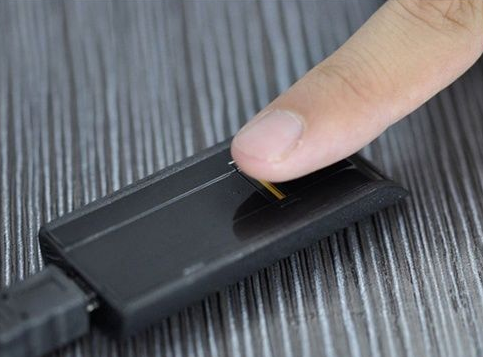
\includegraphics[width=0.3\textwidth]{finger.png}
	\small
	\caption[Leitor biométrico de impressão digital]{Leitor biométrico de impressão digital. Fonte: \cite{ebay}}
	\label{fig:finger}
\end{figure}

Como esses aparelhos requerem investimentos, e na grande maioria dos casos os acessos aos sistemas acontecem de diversos pontos, o uso desses aparelhos se torna inviável.
Dessa forma, alguns sistemas utilizam a combinação das técnicas do uso de senha e de \textit{tokens} para aumentar a segurança dos seus sistemas.
    %---------- Terceiro Capitulo ----------
\chapter{Visão geral da área}\label{cha:visaogeral}

As inovações e evoluções em hardware e software dos dispositivos móveis têm atraído atenção de diversos tipos de pessoas, desde usuários leigos que utilizam poucas funcionalidades desses aparelhos aos pesquisadores que utilizam e se beneficiam da mobilidade e da robustez desses novos dispositivos em parte de seus projetos.

\section{Conectividade}
Os dispositivos móveis encontrados no mercado possibilitam que o usuário possam conectá-lo à Internet de alguma forma, sempre utilizando alguma tecnologia de comunicação sem fio, sendo que as mais comuns são as redes locais sem fio \sigla{WLAN}{Wireless Local Area Network} (\textit{Wireless Local Area Network}) e as redes de telefonia móvel (Celular).
\subsection{WLAN}
Ultimamente o uso da tecnologia de conexão à rede sem fios espalhou-se por todos os lugares, em casa, na universidade, no trabalho, nos aeroportos, hoteis, até em alguns restaurantes.
As redes sem fio são conhecidas como redes Wi-Fi, elas abrangem as tecnologias 802.11 do padrão \sigla{IEEE}{Institute of Electrical and Electronics Engineers} (\textit{Institute of Electrical and Electronics Engineers}).
\begin{citacao}
Wi-Fi é o nome associado à família do padrão IEEE 802.11\footnote{ieee802.org/11/index.shtml}. Assim como o
padrão 802.15, esse padrão opera em faixas de freqüências que não necessitam de licença para instalação e operação. Suas faixas de freqüência são 2,4GHz, 3,6GHz e 5GHz. As aplicações do padrão 802.11 diferem do padrão 802.15 quanto à utilização da rede e a mobilidade do usuário. Wi-Fi oferece alta potência de transmissão e cobre distâncias maiores, oferecendo redes sem fio locais (WLAN). \cite{vanni09}
\end{citacao}
Uma das maiores vantagens das redes Wi-Fi é a sua compatibilidade com praticamente todos os sistemas operacionais, incluindo dipositivos como impressoras e video-games.

As redes Wi-Fi fazem o uso das ondas de rádio para transmitir informações e os dispositivos devem ter um adaptador que traduzem os dados em sinais de rádio. Esses sinais são transmitidos através de uma antena para um decodificador conhecido como roteador, que decodifica os sinais e envia os dados para a Internet através de uma conexão com fios à rede \sigla{LAN}{Local Area Network} (\textit{Local Area Network}).

Como as redes sem fio funcionam recebendo e emitindo sinais, os dados recebidos da Internet são codificados em sinais de rádio pelo roteador e recebidos pelo adaptador do dispositivo conectado como pode ser visto na Figura \ref{fig:wlan}.
Os pontos de acesso às redes Wi-Fi podem ser públicas, como por exemplo nos aeroportos e restaurantes ou fechadas, como nos locais de trabalho e nas casas.

\begin{figure}[!htb]
	\centering
	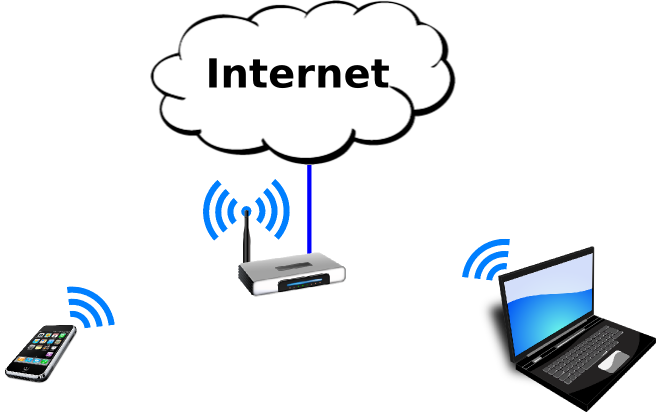
\includegraphics[width=0.45\textwidth]{wlan.png} % <- formatos PNG, JPG e PDF
	\caption[Organização de uma WLAN]{Organização de uma WLAN.}
	\label{fig:wlan}
\end{figure}

Pelo fato de não ser necessário ter acesso físico aos pontos de acesso, qualquer dispositivo com adaptador para redes sem fio poderia ter acesso à Internet através de qualquer roteador Wi-Fi que estivesse no seu alcance. Para bloquear esse acesso às redes Wi-Fi são utilizadas diversas tecnicas de autenticação com protocolos de criptografia como por exemplo:
\begin{itemize}
  \item \sigla{WEP}{Wired Equivalent Privacy} (\textit{Wired Equivalent Privacy})
  - É um algoritmo de segurança que foi introduzido originalmente como parte do protocolo 802.11 que garantiria a confidencialidade dos dados na rede Wi-Fi, mas infelizmente era um algoritmo fácil de quebrar, assim no ano de 2003 a \textit{Wi-Fi Alliance} \footnote{Uma associação da indústria global sem fins lucrativos. wi-fi.org/who-we-are} declarou que o WEP havia sido superado pelo WPA.
  \item \sigla{WPA}{Wi-Fi Protected Access} (\textit{Wi-Fi Protected Access})
  - O WPA e o \sigla{WPA2}{Wi-Fi Protected Access II} (\textit{Wi-Fi Protected Access II}) são dois protocolos de segurança e programas de certificação de segurança desenvolvidos pela \textit{Wi-Fi Alliance} para proteger redes de computadores sem fio. Foram desenvolvidos em resposta às graves deficiências encontradas por pesquisadores no sistema anterior, o WEP.
  \item \sigla{WPS}{Wi-Fi Protected Setup} (\textit{Wi-Fi Protected Setup})
  - Criado pela \textit{Wi-Fi Alliance} e introduzido em 2006, o objetivo deste protocolo é permitir que os usuários domésticos
  possam adicionar novos dispositivos na rede Wi-Fi segura sem a necessidade de entender de protocolos de segurança e sem precisar digitar senhas longas nos dispositivos.
\end{itemize}

\subsection{Telefonia móvel}
A primeira geração de telefones celulares foi lançada na década de 80 e utilizavam o sinal analógico. Eram aparelhos grandes, pouco práticos e inconvinientes para serem carregados pelas pessoas.

Na década de 90 eles foram substituídos pela segunda geração. Os dispositivos móveis passaram a utilizar um sinal digital mais confiável que permitiu o uso de mensagens de texto, ou \sigla{SMS}{Short Message Service} (\textit{Short Message Service}). No entanto, a tecnologia ainda não estava robusta ou rápida o suficiente para lidar com os milhares, e depois milhões, de consumidores que queriam usar telefones celulares. Houve também uma demanda crescente para a transmissão de dados através dos celulares.

A tecnologia 2G não era rápida e confiável o suficiente. Então foi desenvolvida uma tecnologia intermediária, chamada de EDGE ou 2.5G, mas foi com a adoção do 3G que se alcançou rapidez e confiabilidade adequadas para o uso da Internet nos dispositivos móveis.
\begin{citacao}
A tecnologia UMTS (Universal Mobile Telecommunications System), mais conhecida como 3G\footnote{O nome de mercado da tecnologia UMTS está associado a 3G para enfatizar uma evolução das gerações de tecnologias de telefonia celular (1G, 2G, 2.5G); é também conhecida como 3GSM para enfatizar sua estreita ligação com a tecnologia GSM}, foi especificada pelo grupo 3GPP\footnote{O projeto 3GPP é uma iniciativa global com o escopo original de desenvolver especificações e relatórios técnicos para sistemas de Terceira Geração que evoluíssem de redes GSM. Atualmente, o projeto inclui também as tecnologias de acesso GSM/GPRS. Página Web do projeto: 3gpp.org/}

UMTS provê serviços de alta transmissão de dados para redes de dados sem fio e telefonia móvel. Essa tecnologia mantém características da segunda geração GSM para telefonia móvel e \sigla{GPRS}{General Packet Radio Service} (\textit{General Packet Radio Service} para redes de dados sem fio. As novas capacidades incluem envio e recebimento de fotos, gráficos e vídeos, além de serviços de voz e dados. \cite{vanni09}
\end{citacao}

No Brasil estamos vivendo o momento da implantação da tecnologia 4G \sigla{LTE}{Long Term Evolution} (\textit{Long Term Evolution}), uma evolução do 3G que promete velocidades até 10 vezes mais rápida, como pode ser comparado na Tabela \ref{tab:LTE}.

\begin{citacao}
Um dos requisitos do LTE é fornecer taxas de pico downlink de pelo menos 100Mbit/s. A tecnologia permite velocidades acima de 200Mbit/s e a Ericsson já demonstrou taxas acima de 150Mbit/s. Além disso, a latência  deverá ser inferior a 10ms. Efetivamente, isso significa que o LTE – mais do que qualquer outra tecnologia – já atende aos principais requisitos de 4G. \cite{teleco09}
\end{citacao}

\begin{table}[!htb]
	\footnotesize
  	\centering
	\caption[Evolução da Tecnologia GSM -> LTE-Advanced]{Evolução da Tecnologia GSM -> LTE-Advanced. Fonte: \cite{4gamericas}}
	\begin{tabular}{|l|*{8}{c|}}
		\hline \SPACE
		Geração & \multicolumn{4}{|c|}{3G}  & 4G\\ \hline \SPACE
		Tecnologia & WCDMA & HSPA & HSPA+ & LTE & LTE-Advanced\\ \hline \SPACE
		Downlink & 2,0 Mbps & 7,2/14,4 Mbps & 21/42 Mbps & 100Mbps & 1,0 Gbps\\ \hline \SPACE
		Uplink & 474 Kbps & 5,76 Mbps & 7,2/11,5 Mbps & 50 Mbps & 0,5 Gbps\\ \hline \SPACE
		Média teórica & 128-384 kbit/s & 1-10 Mbps & - & - & -\\ \hline \SPACE
		Canalização (MHz) & 5 & 5 & 5 & 20 & 100\\ \hline \SPACE
		Latência (ms) & 250 & ~70 & ~30 & ~10 & <5\\ \hline
	\end{tabular}
	\label{tab:LTE}
\end{table}%\vspace{4cm}

\section{Sistemas operacionais para dispositivos móveis}
Atualmente existem muitas empresas colocando dispositivos móveis no mercado, algumas delas possuem SO próprio enquanto outras optam por um dos SOs diponíveis.
Existem SOs livres e outros de código fechado, alguns são utilizados apenas em dispositivos da própria fabricante, como no caso do IOS da Apple que é utilizado apenas nos iPhones.

\begin{table}[ph]
	\footnotesize
	\centering
	\caption[Sistemas operacionais mais utilizados]{Vendas no mundo de Smartphones para usuários finais por sistema operacional em 2015 (Milhares de Unidades). Fonte: \cite{gartner}}
	\begin{tabular}{|*5{c|}}
		\hline
		\multirow{2}{*}{OS} & \multicolumn{2}{|c|}{\textbf{2015}} & \multicolumn{2}{|c|}{\textbf{2014}}\\ \hhline{~----}
		 & \textbf{Units}  & \textbf{Market Share (\%)} & \textbf{Units}  & \textbf{Market Share(\%)}\\ \hline \SPACE
		Android & 271.010 & 82,2 & 243.484 & 83,8\\ \hline \SPACE
		iOS & 48.086 & 14,6 & 35.345 & 12,2\\ \hline \SPACE
		Windows Phone & 8.198 & 2,5 & 8.095 & 2,8\\ \hline \SPACE
		BlackBerry & 1.153 & 0,3 & 2.044 & 0,7\\ \hline \SPACE
		Others & 1.229 & 0,4 & 1.416,8 & 0,5\\ \hline \SPACE
		Total & 329.676,4 & 100,0 & 290.384,4 & 100,0\\
		\hline
	\end{tabular}
	\label{tab:OS}
\end{table}

A Tabela \ref{tab:OS} apresenta dados de dispositivos móveis por SO, mas estão explícitos apenas os quatro primeiros mais utilizados, logo abaixo é apresentada uma lista com os sistemas operacionais para dispositivos móveis atualmente disponíveis no mercado:

\begin{footnotesize}
	\begin{itemize}
		\item Android
		\begin{itemize}
			\item AOKP
		    \item ColorOS
		    \item CyanogenMod
		    \item Cyanogen OS
		    \item ZenUI
		    \item EMUI
		    \item TouchWiz
		    \item HTC Sense
		    \item Optimus UI
		    \item Fire OS
		    \item Flyme OS
		    \item MIUI
		    \item Nokia X platform
		    \item OxygenOS
		\end{itemize}
	  	\item iOS
		\item Windows 10
		\item BlackBerry 10
		\item Firefox OS
		\item Sailfish OS
		\item Tizen
		\item Ubuntu Touch OS
	\end{itemize}
\end{footnotesize}

Por ser um Software Livre\footnote{Software Livre é uma forma de manifestação de um software em que, resumidamente, permite-se adaptações ou modificações em seu código de forma espontânea, ou seja, sem que haja a necessidade de solicitar permissão ao seu proprietário para modificá-lo.} e poder ser modificado livremente, o Android apresenta essa sub-lista de sistemas. Essas modificações são realizadas por outras empresas que utilizam o sistema modificado em seus produtos como por exemplo em aparelhos celulares, \textit{tablets}, TVs, \textit{smartwatches} e até \textit{desktops}.
    %---------- Quarto Capitulo ----------
\chapter{Ferramentas de desenvolvimento}\label{cha:ferramentas}

\section{Linguagens de Programação e Frameworks de Desenvolvimento}
As organizações Google, Apple e Microsoft que desenvolvem os sistemas operacionais Android, iOS e Windows, respectivamente, oferecem aos desenvolvedores ferramentas e ambientes de desenvolvimento, conhecidos como IDE (\textit{Integrated Development Environment}), ricos em bibliotecas que fornecem suporte e facilidades no desenvolvimento de aplicativos e também mantêm sites voltados aos desenvolvedores com documentos e informações sobre como utilizar as bibliotecas e as ferramentas para o desenvolvimento de aplicativos.

Além das IDE e dos \sigla{SDK}{Software Development Kit} (\textit{Software Development Kit}) disponibilizados por essas empresas, outras organizações também desenvolvem tecnologias que apoiam a criação de aplicativos para essas platafomas como por exemplo as empresas Appcelerator e Apache. A Appcelerator disponibiliza um ambiente de desenvolvimento completo com IDE, plugins e bibliotecas conhecido como Titanium IDE, já a Apache disponibiliza aos desenvolvedores uma plataforma para criar aplicativos chamada Cordova que utiliza as tecnologias Javascript, \sigla{HTML}{Hyper Text Markup Language} (\textit{Hyper Text Markup Language}) e \sigla{CSS}{Cascading Style Sheets} (\textit{Cascading Style Sheets}).

Javascript é a linguagem com o maior número de repositórios ativos no GitHub, como mostrado na Figura \ref{fig:javascript}.

\begin{figure}[!htb]
	\centering
	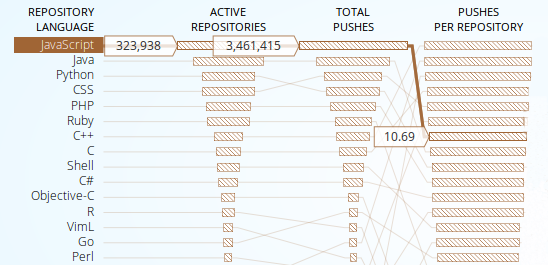
\includegraphics[width=.8\textwidth]{javascript-st.png} % <- formatos PNG, JPG e PDF
	\caption[Linguagens com maior número de repositórios ativos no GitHub]{Gráfico sobre as linguagens com repositórios ativos no GitHub. Fonte: \cite{githut}}
	\label{fig:javascript}
\end{figure}
\vspace{-3mm}

Com esse grande número de repositórios, a linguagem Javascript torna-se uma opção muito atrativa na escolha como linguagem principal no desenvolvimento de aplicativos, pois existem muitas pessoas utilizando a linguagem e isso faz com que seja fácil de encontrar exemplos de uso de código, existe a facilidade na obtenção de respostas de dúvidas em foruns de discussão, e também acontece o aumento na quantidade de bibliotecas utéis que podem ser utilizadas em diversos tipos de projetos.

\subsection{\normalfont\itshape Frameworks utilizando Apache Cordova}
Várias outras organizações utilizam o Apache Cordova como núcleo em seus frameworks para o desenvolvimento de aplicativos para dispositivos móveis, como é o caso do Adobe PhoneGap, Intel XDK e Ionic Framework.

Segundo a documentação do Apache Cordova, o \textit{framework} oferece uma camada entre as várias funcionalidades existentes nos dispositivos móveis.
\begin{citacao}
O Cordova fornece uma interface que permite a comunicação entre os componentes nativos e o seu \textit{plugin}. Isso possibilita a chamada das funcionalidades nativas através do Javascript. Idealmente, a \sigla{API}{Application Program Interface} (\textit{Application Program Interface}) Javascript para a invocação de código nativo seria consistente para múltiplas plataformas. \cite{cordova}
\end{citacao}

A documentação do Apache Cordova mostra como criar um projeto simples através de poucos comandos e um desses comandos é a adição das plataformas suportadas, onde o desenvolvedor pode adicionar plataformas alvo e no momento da compilação serão gerados artefatos que poderão ser instalados nas plataformas correspondentes.
A documentação também apresenta uma tabela que exibe quais são as plataformas suportadas e quais as funcionalidades nativas que podem ser chamadas através de seu plugin.
Na Tabela \ref{tab:cordova} é exibido um resumo da tabela do Cordova e como pode ser notado, são poucas as funcionalidades que não são suportadas, isso aumenta as chances do uso desse \textit{framework}, já que com uma única implementação podemos ter várias plataformas alvo.

\begin{table}[!htb]
	\footnotesize
	\centering
	\caption[Funcionalidades nativas suportadas pelo \textit{plugin} Cordova]{Algumas das funcionalidades nativas suportadas pelo \textit{plugin} Cordova}
	\begin{tabular}{*8{c|}}
		 & \textbf{FireOS} & \textbf{Android} & \textbf{Blackberry} & \textbf{Firefox OS} & \textbf{iOS} & \textbf{Ubuntu} & \textbf{Windows}\\ \hline
		Accelerometer & \checkmark & \checkmark & \checkmark & \checkmark & \checkmark & \checkmark & \checkmark\\ \hline \SPACE
		Camera & \checkmark & \checkmark & \checkmark & \checkmark & \checkmark & \checkmark & \checkmark\\ \hline \SPACE
		Compass & \checkmark & \checkmark & \checkmark & x & \checkmark & \checkmark & \checkmark\\ \hline \SPACE
		Status Bar & x & \checkmark & x & x & \checkmark & x & \checkmark\\ \hline \SPACE
		Geolocalization & \checkmark & \checkmark & \checkmark & \checkmark & \checkmark & \checkmark & \checkmark\\ \hline \SPACE
		Events & \checkmark & \checkmark & \checkmark & x & \checkmark & \checkmark & \checkmark\\ \hline \SPACE
		BatteryStatus & \checkmark & \checkmark & \checkmark & \checkmark & \checkmark & x & \checkmark\\
		\hline
	\end{tabular}
	\label{tab:cordova}
\end{table}

As aplicações que são desenvolvidas com essas tecnologias funcionam sobre o navegador de Internet dos dispositivos, isso faz com que nem todo o tipo de aplicação possa se beneficiar dessas facilidades. Aplicações que necessitam de um desempenho maior deverão ser implementadas em código nativo.

\subsection{Javascript em qualquer lugar}
Javascript está se tornando muito popular também como linguagem de backend, com o Node.Js.

Logo abaixo é apresentado um exemplo de código Node.js, extraído da documentação e que pode ser encontrado em \cite{nodejs}. Esse pequeno trecho de código quando executado disponibilizá um servidor web que poderá manipular muitas conexões concorrentemente.
\begin{verbatim}
	  const http = require('http');
	  const hostname = '127.0.0.1';
	  const port = 1337;
	  http.createServer((req, res) => {
	      res.writeHead(200, { 'Content-Type': 'text/plain' });
	      res.end('Hello World\n');
	  }).listen(port, hostname, () => {
	      console.log(`Running at http://${hostname}:${port}/`);
	  });
\end{verbatim}

Caso esse código seja executado e alguém aponte o navegador de internet para o endereço do servidor, ele apenas devolverá ao usuário a mensagem \textit{Hello World}. Nada muito útil, mas o que deve ser levado em consideração aqui é essa simplicidade e poder que o Node.js apresenta.

O Javascript pode ser encontrado até como linguagem auxiliar para manipulação de dados em Banco de Dados, como é o caso do MongoDB, um banco de dados orientado a documentos que utiliza o \sigla{JSON}{JavaScript Object Notation} (\textit{JavaScript Object Notation}) como estrutura de dados.
No SGBD desse banco de dados podemos utilizar funções Javascript sobre os dados retornados numa consulta.
    %---------- Quinto Capitulo ----------
\chapter{Desenvolvimento}\label{cha:desenvolvimento}
Este trabalho de conclusão de curso necessitou que fossem implementados uma aplicação servidora, o \textit{Broker}, que gerencia a escolha das aplicações que melhor atendem as configurações definidas pelo usuário; a aplicação para dispositivo móvel, onde o usuário realiza as configurações que deseja para cada tipo de serviço e que também consome esses serviços; e também alguns simuladores de provedores de serviço. Para armazenamento de dados, foi utilizado um banco de dados na nuvem. A Figura \ref{fig:arquitetura} mostra a organização da arquitetura do projeto.

\begin{figure}[!htb]
  \centering
  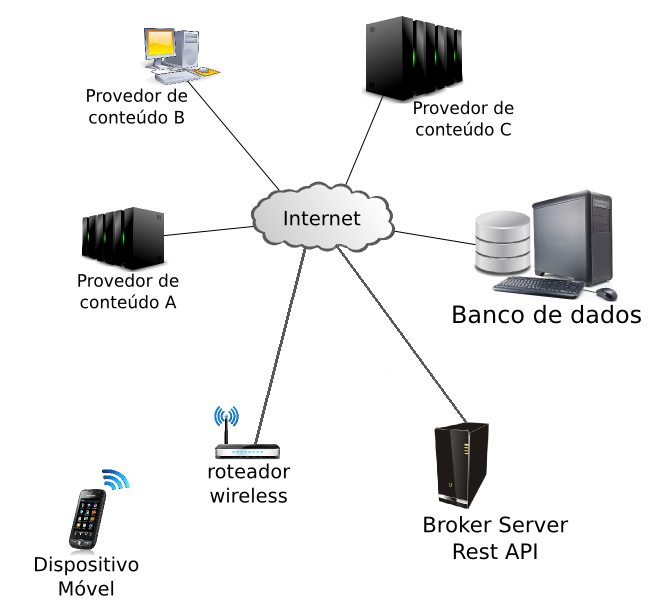
\includegraphics[width=.7\textwidth]{arquitetura.png} % <- formatos PNG, JPG e PDF
  \caption[Arquitetura do projeto]{Arquitetura do projeto}
  \label{fig:arquitetura}
\end{figure}

%----------------- Serviços -----------------
\section{Serviços}
Os dispositivos móveis são utilizados diariamente como 'computadores de bordo' pelas pessoas, são meios de obter informações sobre o que está acontecendo. No decorrer do dia a pessoa utiliza seu dispositivo para consultar email, trocar mensagens, consultar as condições do trânsito, condições climáticas, ler notícias do jornal, obter rotas, ouvir música e muito mais.

Muitos desses serviços necessitam que o usuário tenha uma conta registrada e que seja autenticado antes de utilizá-lo. E também são genéricos o suficiente para oferecer o serviço ao maior número de usuários possíveis.

Devido a essa característica de oferecer um serviço genérico, o usuário deve aplicar filtros na aplicação do serviço para obter a informação necessária.

Vamos utilizar como exemplo uma consulta ao serviço de metereologia, então o usuário:
\begin{footnotesize}
  \begin{enumerate}
  \item Abre o navegador de internet;
  \item Abre um site de busca;
  \item Procura pela palavra metereologia;
  \item Escolhe um dos serviços na lista;
  \item Tenta usar o serviço, se não conseguir volta ao passo anterior;
  \item Se necessário, cria uma conta e autentica-se no serviço;
  \item Aplica os filtros necessários;
  \item Obtém as informações.
  \end{enumerate}
\end{footnotesize}

Dependendo do tipo de serviço, esses passos serão sempre repetidos, principalmente o passo de autenticação, e as informações do usuário vão estar sempre expostas numa rede sem fio onde qualquer pessoa mal intensionada, com ferramentas adequadas, poderá capturá-las. E é esse tipo de problema que queremos resolver.

\subsection{Implementação de um serviço como prova de conceito}
Como as implementações dos serviços não fazem parte do escopo deste trabalho, foram implementados apenas serviços incompletos que simulam o funcionamento de um serviço real. No caso, foram implementados três serviços que oferecem dados metereológicos falsos, sendo que em um deles é necessário que o usuário tenha sido previamente cadastrado, assim para obter as informações do serviço, precisará realizar a autenticação.

Esses serviços foram implementados como \textit{Web Services} \sigla{REST}{Representational State Transfer} (\textit{Representational State Transfer}), assim precisamos apenas realizar uma chamada à interface adequada para obter a resposta.

Existem provedores de serviços reais que oferecem esse tipo de API, como por exemplo o \textit{OpenWeatherMap}\footnote{openweathermap.org/api}, não é gratuito e é um serviço rico em informações. Para utilizar o serviço pode ser realizado um cadastro simples que possui um uso limitado, nesse cadastro o usuário recebe uma chave que pode ser usado numa requisição como no exemplo a seguir:

\url{http://api.openweathermap.org/data/2.5/weather?q=Maringa,br&APPID=CHAVE_DO_USUARIO}

Essa consulta retornaria um JSON com muitas informações da cidade de Maringá, logo abaixo pode ser visto um resumo dessas informações:

\begin{footnotesize}
  \begin{verbatim}
      { "coord":{
          "lon": -51.94
          "lat": -23.43
        }, "weather": {
          "description": "light rain",
          "temp": 30,
          "pressure": 1011,
          "humidity": 74,
          "temp_min": 30,
          "temp_max": 30,
          "wind": {
            "speed": 2.1
          }, "sys": {
            "name": "Maringa",
            "country": "BR"
          }
        }
      }
  \end{verbatim}
\end{footnotesize}

Os serviços que foram implementados para este trabalho seguem uma linha semelhante, eles respondem a requisições POST nos endereços:
\begin{footnotesize}
  \begin{enumerate}
  \item \url{http://weather-provider.herokuapp.com/weather}
  \item \url{http://weather-nd-provider.herokuapp.com/weather}
  \item \url{http://weather-rd-provider.herokuapp.com/weather}
  \end{enumerate}
\end{footnotesize}

Sendo que o primeiro necessita que o usuário seja registrado no serviço e que realize a autenticação para poder utilizá-lo. Para realizar o registro no serviço é necessário uma chamada simples à interface de registro:

\url{http://weather-provider.herokuapp.com/register/EMAIL_DO_USUARIO/UMA_SENHA}

Como já foi dito, a implementação dos serviços não fazem parte do escopo do trabalho, então foram criadas apenas as interfaces REST necessárias para o funcionamento. Assim, as chamadas às interfaces destes serviços respondem com uma lista com objetos JSON com dados fictícios sobre o clima de algumas cidades do Paraná. Como no exemplo logo abaixo:

\begin{footnotesize}
  \begin{verbatim}
  [{  "provider": "First Weather Provider",
      "city": "Curitiba",
      "temperature": 15,
      "Humidity": 47,
      "sky": "weather-cloudy",
      "update": "2016-01-28T03:06:06.756Z"
  },{ "provider": "First Weather Provider",
      "city": "Maringá",
      "temperature": 7,
      "Humidity": 33,
      "sky": "weather-rainy",
      "update": "2016-01-28T18:12:10.002Z"
  },{ "provider": "First Weather Provider",
      "city": "Londrina",
      "temperature": 9,
      "Humidity": 6,
      "sky": "weather-cloudy",
      "update": "2016-01-28T06:06:10.021Z"
  },{ "provider": "First Weather Provider",
      "city": "Foz do Iguaçu",
      "temperature": 31,
      "Humidity": 94,
      "sky": "weather-rainy",
      "update": "2016-01-28T16:08:08.096Z"
  },{ "provider": "First Weather Provider",
      "city": "Guarapuava",
      "temperature": -1,
      "Humidity": 98,
      "sky": "weather-snowy",
      "update": "2016-01-28T03:11:11.238Z"
  }]
  \end{verbatim}
\end{footnotesize}

Ao obter esses dados, o \textit{Broker} trabalhará sobre eles e escolherá as informações do serviço que melhor atendem às preferências do usuário.

\subsection{Serviços disponíveis}
O \textit{Broker} entrega à aplicação do dispositivo móvel uma lista com alguns tipos de serviços e seus atributos de preferências, que são:

\begin{footnotesize}
  \begin{itemize}
    \item Games
      \begin{itemize}
        \item Amount of users
      \end{itemize}
    \item Video
      \begin{itemize}
        \item Amount of videos
      \end{itemize}
    \item News
      \begin{itemize}
        \item City
        \item Last update
        \item Closer to me
      \end{itemize}
    \item Music
      \begin{itemize}
        \item Amount of music
      \end{itemize}
    \item Weather
      \begin{itemize}
        \item City
        \item Last update
      \end{itemize}
  \end{itemize}
\end{footnotesize}

%----------------- Aplicação -----------------
\section{A aplicação para dispositivos móveis}
A implementação do aplicativo para dispositivo móvel utilizou o Ionic \textit{Framework}. Dessa forma, a aplicação foi desenvolvida com o uso das Linguagens Javascript, HTML e CSS.

O Ionic \textit{Framework} foi desenvolvido sobre outro \textit{framework}, o Apache Cordova, o que idealmente permite que a aplicação desenvolvida possa ser executada em todas as plataformas de dispositivo móvel à qual o Apache Cordova oferece suporte.

Abaixo é apresentada a Figura \ref{fig:ionicarch} que mostra a organização da arquitetura do \textit{framework}. Essa figura é meramente ilustrativa, pois nas últimas camadas temos um número bem maior de funcionalidades nos dispositivos, assim como um número maior de sistemas operacionais alvos do Apache Cordova.

\begin{figure}[!htb]
  \centering
  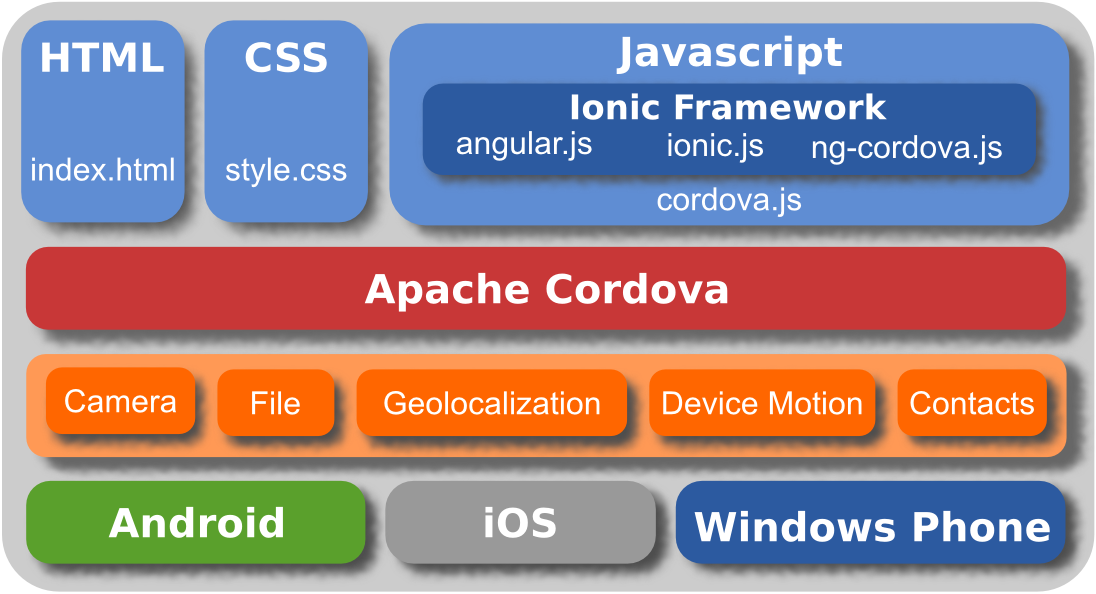
\includegraphics[width=.8\textwidth]{ionicarch.png} % <- formatos PNG, JPG e PDF
  \caption[Arquitetura do Ionic Framework]{Arquitetura do Ionic Framework}
  \label{fig:ionicarch}
\end{figure}

A implementação e os testes da aplicação tiveram como SO alvo apenas o Android.

A aplicação foi desenvolvida com uma interface intuitiva, com ícones expressivos para que o usuário tivesse uma experiência agradável e sem transtornos.

As configurações necessárias são mínimas e qualquer pessoa envolvida no contexto da aplicação conseguiria realizá-las em poucos passos e já teria a aplicação em funcionamento em seu aparelho.

O Apêndice A apresenta um modelo de navegação na aplicação.

\subsection{Configurando um serviço}
Como o objetivo da aplicação no dispositivo móvel é apresentar ao usuário o melhor serviço que respeite as suas preferências, é necessário que esses atributos sejam cadastrados de alguma forma. Nos passos a seguir será mostrado como configurar um desses serviços, no caso, será utilizado o serviço de metereologia (\textit{Weather}).

Depois de realizar as configurações iniciais, como:
\begin{footnotesize}
  \begin{enumerate}
    \item cadastrar o endereço do \textit{Broker};
    \item cadastrar o usuário;
    \item realizar \textit{login} na aplicação
  \end{enumerate}
\end{footnotesize}

o usuário navegará até a aba de serviços, exibido na Figura \ref{fig:navegar}

\begin{figure}[!htb]
  \centering
  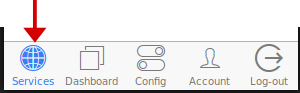
\includegraphics[width=.4\textwidth]{navegar.png} % <- formatos PNG, JPG e PDF
  \caption[Aba de serviços]{Aba de serviços}
  \label{fig:navegar}
\end{figure}

o usuário deverá tocar no botão de configuração do endereço do provedor de serviço, em destaque na Figura \ref{fig:configurl}

\begin{figure}[!htb]
  \centering
  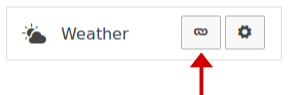
\includegraphics[width=.5\textwidth]{configurl.png} % <- formatos PNG, JPG e PDF
  \caption[Botão para configuração dos endereços dos serviços]{Botão para configuração dos endereços dos serviços}
  \label{fig:configurl}
\end{figure}

e realizar a configuração do endereço, preenchendo os campos como os exibidos na Figura \ref{fig:registerurl}, se necessário, adicionar os dados de autenticação do provedor de serviço.

\begin{figure}[!htb]
  \centering
  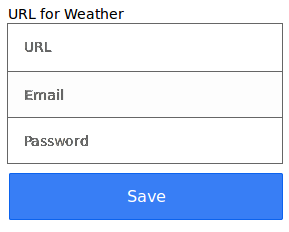
\includegraphics[width=.4\textwidth]{registerurl.png} % <- formatos PNG, JPG e PDF
  \caption[Cadastro do endereço do provedor de serviço]{Cadastro do endereço do provedor de serviço}
  \label{fig:registerurl}
\end{figure}

Logo em seguida, o usuário deverá configurar suas preferências, tocando no botão em destaque na Figura \ref{fig:configprefs}

\begin{figure}[!htb]
  \centering
  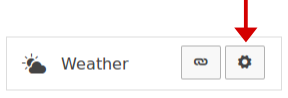
\includegraphics[width=.5\textwidth]{configprefs.png} % <- formatos PNG, JPG e PDF
  \caption[Botão para configuração das preferências do usuário]{Botão para configuração das preferências do usuário}
  \label{fig:configprefs}
\end{figure}

e realizar a configuração das preferências, que no caso para o tipo de serviço \textit{Weather} o usuário marcará se precisa que as informações sejam as mais atualizadas possíveis e qual a sua cidade de preferência, como mostrado na Figura \ref{fig:weatherprefs}

\begin{figure}[!htb]
  \centering
  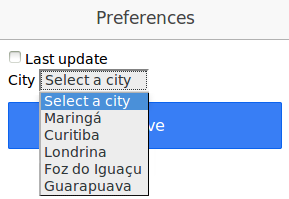
\includegraphics[width=.4\textwidth]{weatherprefs.png} % <- formatos PNG, JPG e PDF
  \caption[Configuração das preferências do usuário]{Configuração das preferências do usuário}
  \label{fig:weatherprefs}
\end{figure}

Cadastrando esses dados, o usuário não precisará mais informar o endereço do provedor de serviço nem seus dados de autenticação, ele será autenticado de forma transparente e receberá na aba \textit{Dashboard}, em destaque na Figura \ref{fig:dashboard}, as informações do provedor que melhor atender as suas preferências.

\begin{figure}[!htb]
  \centering
  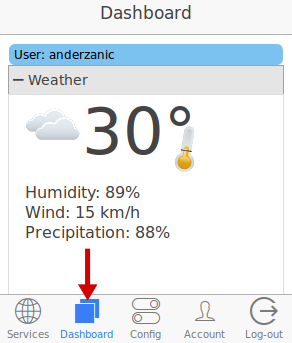
\includegraphics[width=.4\textwidth]{dashboard.png} % <- formatos PNG, JPG e PDF
  \caption[Aba \textit{Dashboad} que exibe os serviços configurados]{Aba \textit{Dashboad} que exibe os serviços configurados}
  \label{fig:dashboard}
\end{figure}

Nessa aba são exibidos apenas os serviços que tiveram as preferências configuradas.

\subsection{Angular.js}
Angular.js foi desenvolvido pela Google. É um \textit{framework} para desenvolvimento de aplicações web \textit{Single Page Applications}, onde todas as páginas da aplicação são desenvolvidas como \textit{templates} e são injetadas na página principal quando requisitadas.

Uma característica muito importante do Angular.js é que ele estende o vocabulário padrão do HTML, permitindo que sejam desenvolvidos sistemas com um código muito mais expressivo no \textit{front-end}.

Como por exemplo o uso de uma \textit{tag} HTML como: 
\begin{footnotesize}
  \begin{verbatim}
                  <genero />
  \end{verbatim}
\end{footnotesize}

é mais expressivo do que:

\begin{footnotesize}
  \begin{verbatim}
                  <label>Gênero: </label>
                  <select name="genero">
                    <option value="M">Masculino</option>
                    <option value="F">Feminino</option>
                  </select>
  \end{verbatim}
\end{footnotesize}

Além desse ganho na expressividade, a modularização e reúso de código acontece efetivamente, o que diminui o tempo de desenvolvimento e aumenta a qualidade das aplicações.

Outro recurso muito interessante é o \textit{Two-Way Data Binding}, que permite a sincronização automática dos dados da \textit{view} com o modelo sem a manipulação direta do DOM pelo desenvolvedor.

\begin{figure}[!htb]
  \centering
  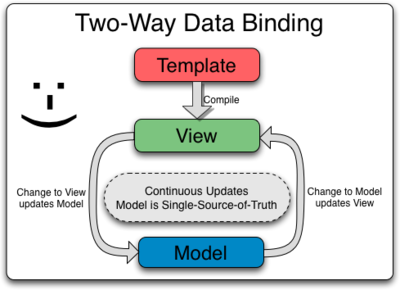
\includegraphics[width=.5\textwidth]{databinding.png} % <- formatos PNG, JPG e PDF
  \caption[Sincronização automática do \textit{model} e da \textit{view}]{Sincronização automática do \textit{model} e da \textit{view}. Fonte: \cite{angulardb}}
  \label{fig:twoway}
\end{figure}

\subsection{Construção dinâmica de formulário}
Um dos desafios enfrentados durante a implementação da aplicação para o dispositivo móvel foi a construção do formulário que exibe as configurações das preferências do usuário para cada serviço. Como cada serviço apresenta um determinado conjunto de atributos, iria ser necessário a implementação de uma \textit{template} para cada tipo de serviço, isso iria aumentar a complexidade de atualizações e manutenções de código.

Para evitar esses problemas e outros que poderiam surgir, como por exemplo: uma mudança nos atributos do serviço, foi desenvolvido um componente, que constrói o formulário de configuração de preferências de acordo com parâmetros enviados pelo \textit{Broker}.

Por exemplo, podemos enviar essas configurações abaixo ao dispositivo móvel e ele produzirá um formulário como a Figura \ref{fig:geracaoauto}.
\begin{footnotesize}
  \begin{verbatim}
          { "element": "input",
            "type": "text",
            "name": "email",
            "label": "Email"
          },
          { "element": "input",
            "type": "password",
            "name": "password",
            "label": "Password" }
  \end{verbatim}
\end{footnotesize}

\begin{figure}[!htb]
  \centering
  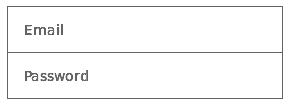
\includegraphics[width=.4\textwidth]{geracaoauto.png} % <- formatos PNG, JPG e PDF
  \caption[Geração automática de formulário]{Geração automática de formulário}
  \label{fig:geracaoauto}
\end{figure}

%----------------- Broker -----------------
\section{O \normalfont\itshape Broker}
O \textit{Broker} foi implementado como um \textit{Web Services} REST que expõe as interfaces necessárias para a aplicação cliente instalada no dispositivo móvel.
\begin{citacao}
O estilo REST é uma abstração dos elementos arquitectônicos dentro de um sistema hipermídia distribuído. REST ignora os detalhes da implementação do componente e da sintaxe do protocolo, a fim de se concentrar nos papéis dos componentes, as restrições sobre a sua interação com outros componentes, e sua interpretação de dados significativos. Ela abrange as restrições fundamentais sobre os componentes, conectores e dados que definem a base da arquitetura Web e, portanto, a essência do seu comportamento como um aplicativo baseado na rede. \cite{fielding2000architectural}
\end{citacao}
Em outras palavras, REST é um alternativa leve para \textit{Web Services} pois ele expõe apenas interfaces com os métodos padrão do \sigla{HTTP}{Hypertext Transfer Protocol} (\textit{Hypertext Transfer Protocol}), que também são conhecidos como verbos: GET e POST. Além desses dois existem os PUT, DELETE, HEAD e OPTIONS\footnote{O significado de cada um desses métodos é definido na especificação do HTTP, juntamente com algumas garantias sobre o seus comportamentos}.

As interfaces que o servidor \textit{Broker} expõe aceitam e respondem objetos JSON, como por exemplo uma chamada GET ao método \textit{types} que responde uma lista com os tipos de serviços disponíveis e suas configurações.
Se fizermos essa requisição \url{http://brokerserver.herokuapp.com/types} à API REST, teremos como resultado uma lista de objetos JSON como no exemplo abaixo:
\begin{footnotesize}
  \begin{verbatim}
    [{ "_id": "5605df14e4b0eeb9ac04606c",
       "type": "Weather",
       "icon": "icon ion-ios-partlysunny",
       "url": "#/weather",
       "preferences": [
         { "element": "input",
           "type": "checkbox",
           "name": "last",
           "label": "Last update"
         },{ "element": "input",
           "type": "text",
           "name": "city",
           "label": "City"
         } ]
     },{"_id": "5605df22e4b0eeb9ac04606d",
      "type": "Music",
      "icon": "icon ion-music-note",
      "url": "#/music",
      "preferences": [
        { "element": "input",
          "type": "number",
          "name": "amount",
          "label": "Amount of music"
        } ]
  } ]
  \end{verbatim}
\end{footnotesize}
\vspace{-7mm}

No evento de \textit{login} da aplicação do dispositivo móvel, é feita uma chamada POST ao método \textit{login} do \textit{Broker}, os parâmetros são enviados ao servidor no corpo da mensagem, como podemos notar na Figura \ref{fig:logindebug}, onde a aplicação foi executada em um navegador de internet com o console de \textit{debug} aberto.

\begin{figure}[h]
  \center
  \subfigure{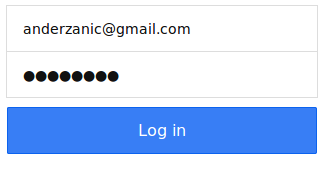
\includegraphics[width=.4\textwidth]{login.png}}
  \qquad
  \subfigure{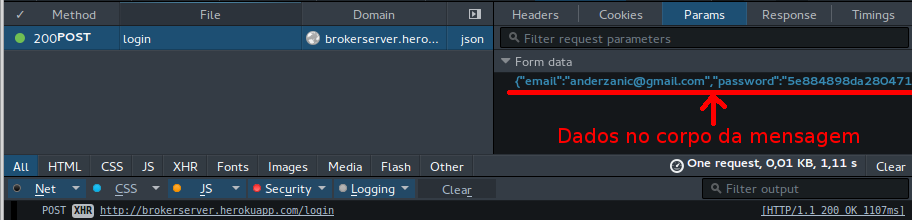
\includegraphics[width=1.1\textwidth]{debug.png}}
  \caption[\textit{Debug} da simulação de um \textit{login} na aplicação móvel]{\textit{Debug} da simulação de um \textit{login} na aplicação móvel}
  \label{fig:logindebug}
\end{figure}

Ao apertar o botão \textit{'Log in'} na aplicação móvel, a \sigla{URL}{Uniform Resource Locator} (\textit{Uniform Resource Locator}) \url{
http://brokerserver.herokuapp.com/login} foi chamada com os parâmetros \textit{email} e \textit{password} sendo enviados no corpo da mensagem.

\subsection{Plugar novos serviços}
O \textit{Broker} é o sistema encarregado de realizar a análise das preferências do usuário e deve cruzar essas informações com os estados dos provedores de serviço para poder decidir qual é o serviço que melhor atende aos requisitos do usuário.

Dependendo da linguagem de programação escolhida para resolver esse tipo de problema, pode ser que sejam necessárias muitas linhas de código para que seja alcançado um algoritmo adequado.

A característica funcional do Javascript foi um fator relevante pois foram utilizadas funções de alta ordem, funções que podem ser passadas como parâmetros para outras funções, e elas auxiliaram na resolução do problema com um código simples, limpo e elegante. Abaixo temos um exemplo do uso de funções de alta ordem em Javascript.

Suponha que temos uma lista de objetos e é preciso escolher um desses objetos, em Javascript podemos implementar uma função que funcionará como um predicado, e todos os objetos que responderem \textit{"verdade"} a esse predicado, serão escolhidos.

\begin{footnotesize}
  \begin{verbatim}
      var lista = [ {"cidade": "Maringá", "Estado":"PR"},
                    {"cidade": "Curitiba", "Estado":"PR"} ];
      var predicado = function(candidato){
                        return candidato.cidade === "Maringá";
                      };
      var resultado = lista.filter(predicado);
      console.log(resultado);
      // Imprime no console: [{"cidade": "Maringá", "Estado":"PR"}]
  \end{verbatim}
\end{footnotesize}

Esse é um exemplo bem simples, mas a função de predicado pode ter a complexidade necessária e ainda assim o código que aplica o predicado se manterá sempre simples e além disso essa função poder ser modularizada transformado-se em um \textit{plugin} que poderá ser aplicado onde for necessário.

No caso do \textit{Broker} isso foi fundamental pois cada vez que um novo serviço for ser oferecido será apenas necessário implementar o predicado, baseado nos atributos do serviço, e realizar o registro desse novo predicado no servidor, com a adição de uma única linha de código:

\begin{footnotesize}
  \begin{verbatim}
      var novoservico = require('./novoservico.js');
  \end{verbatim}
\end{footnotesize}

\subsection{Jasmine \normalfont\itshape Framework}
Jasmine é um \textit{framework} para testes de códigos Javascript.
\begin{citacao}
Jasmine é um framework de testes \sigla{BDD}{Behavior Driven Development} (\textit{Behavior Driven Development}) para JavaScript. Ele não depende de navegadores, \sigla{DOM}{Document Object Model} (\textit{Document Object Model}), ou qualquer \textit{framework} JavaScript. Jasmine é adequado para websites, projetos Node.js, ou em qualquer lugar que o JavaScript possa ser executado.\cite{jasmine}
\end{citacao}

Como Javascript é uma linguagem de tipagem dinâmica, é necessário que sejam implementados testes que possam aumentar a confiança de que as funções estão respondendo de maneira correta.
Dessa forma, algumas funções do \textit{Broker} tiveram testes implementados.

O \textit{framework} Jasmine suporta a técnica ágil "Desenvolvimento Guiado por Comportamento", conhecido pela sigla em inglês BDD, é uma técnica que encoraja o envolvimento entre os desenvolvedores, setores de qualidade e pessoas sem conhecimento técnico e que dominam a regra do negócio. Os testes são criados utilizando a linguagem nativa e a codificação do teste em Javascript, o uso da linguagem nativa auxilia o desenvolvedor a manter o foco na razão pela qual o código deve ser implementado.
Abaixo temos um exemplo de um teste com Jasmine:
\begin{footnotesize}
  \begin{verbatim}
  describe("serviços disponíveis", function() {
    beforeEach(function() {
      jasmine.Ajax.install();
      jasmine.Ajax.stubRequest('http://weather-provider.herokuapp.com/weather')
        .andReturn({
          responseText: { "provider": "Weather Provider",
                          "city": "Maringá",
                          "temperature": 29,
                          "Humidity": 48,
                          "sky": "weather-sunny",
                          "update": "2016-02-10T18:23:44.479Z" };
        });
    });
    afterEach(function() {
      jasmine.Ajax.uninstall();
    });
    it("a temperatura de Maringá deverá ser exibida", function() {
      $.ajax({
        url: 'http://weather-provider.herokuapp.com/weather'
      }).success(result){
        expect(result.city).toEqual('Maringá');
        expect(result.temperatura).toEqual(29);
      };
    });
  });
  \end{verbatim}
\end{footnotesize}

Antes da execução de cada teste, que está implementado dentro de cada declaração "it('mensagem', function(){});", é executado o código declarado na função 'beforeEach'. Isto cria um ambiente que responderá às chamadas Ajax no endereço 'http://weather-provider.herokuapp.com/weather' com a resposta declarada em 'responseText'.

No final da execução de cada teste o trecho 'afterEach' é executado destruindo o ambiente criado.

Esses ambientes são conhecidos como \textit{Mocks} e servem para isolar o teste no que realmente deve ser testado, no caso do exemplo, se a chamada Ajax não fosse um ambiente falso, ela tentaria realizar uma requisição, isso dependeria de conexão à internet, do endereço que está sendo chamado ter um servidor ativo. São muitas variáveis a serem controladas e desnecessárias para um teste unitário.

\section{Ferramentas}
\subsection{MongoLab}
O banco de dados utilizado foi o MongoDB, e como SGBD foi escolhido o MongoLab.
O MongoLab pode ser acessado através do endereço \url{http://mongolab.com} é um serviço de banco de dados online que oferece diversos pacotes de soluções para MongoDB com diversos preços, desde o pacote gratuito com algumas restrições de uso até pacotes com valores de USD 5890.00.

O MongoLab oferece recursos para a manipulação e gerenciamento dos dados através de:
\begin{footnotesize}
  \begin{itemize}
  \item uma interface web;
  \item chamadas à API REST;
  \item conexões por \textit{driver};
  \end{itemize}
\end{footnotesize}

Para o \textit{Broker} foi configurado o uso de \textit{driver} de conexão, pois ele apresenta o melhor desempenho das opções existentes.

\subsection{Heroku}
Heroku é um serviço de hospedagem de aplicações que também possue os pacotes gratuito e pagos. A forma de cobrança do Heroku é diferente, a cobrança acontece de acordo com o uso de processamento e requisições de suas aplicações.

Ele possui uma aplicação cliente que permite monitorar e controlar suas aplicações, além da interface web que também permite o controle das aplicações.

Uma funcionalidade muito interessante do Heroku é a integração com o GitHub que permite o \textit{deploy} automático das aplicações assim que as alterações são versionadas em uma determinada \textit{branch}.

\subsection{GitHub}
O Git foi escolhido como o sistema de controle de versão das aplicações móvel e servidora e até deste documento. E o GitHub foi o escolhido como plataforma de hospedagem.
O GitHub permite a criação gratuita de repositórios públicos e possui ferramentas na plataforma web que permitem gerenciar e monitorar os repositórios.
Na lista abaixo temos os endereços dos repositórios que podem ser clonados:

\begin{footnotesize}
  \begin{itemize}
  \item[TCC:] \url{https://github.com/andersonzanichelli/tcc-latex.git}
  \item[Broker:] \url{https://github.com/andersonzanichelli/brokerserver.git}
  \item[Cliente:] \url{https://github.com/andersonzanichelli/brokerclientapp.git}
  \end{itemize}
\end{footnotesize}

\subsection{NPM e Bower}
Assim como as aplicações Java contam com o Maven ou Gradle como ferramentas de gerenciamento de dependências, Javascript tem o \sigla{NPM}{Node.js Package Manager} (\textit{Node.js Package Manager}). Para dependências de \textit{front-end} foi utilizado o Bower.
Gerenciadores de dependências são ferramentas incríveis que configuram um ambiente de desenvolvimento, de teste ou de produção automaticamente e de forma padronizada, com as versões corretas de cada dependência.
    %---------- Sexto Capitulo ----------
\chapter{Conclusões e Trabalhos Futuros}\label{cha:conclusao}

\section{Conclusões}
Os dispositivos móveis devem ser vistos como ferramentas que auxiliam e facilitam a vida do usuário. Como facilitadores do dia-a-dia, estas ferramentas devem possuir aplicativos que evitem expor as informações do usuário a riscos desnecessários e que apresente ao usuário serviços que realmente sejam de utilidade.

Cada tipo de serviço apresenta um conjunto de atributos que são relevantes para o usuário no momento da escolha do serviço e conhecendo previamente quais são os valores de cada atributo, para cada usuário, essa escolha pode ser automatizada.

Este foi o objetivo deste trabalho de conclusão de curso, a implementação de aplicações que permitam a configuração desses atributos relevantes e a escolha automática do serviço baseando-se nas configurações.

Assim foi necessário a implementação de uma aplicação para dispositivos móveis onde o usuário configura quais são os valores para os atributos de cada tipo de serviço e que também, além de interface de configuração, é a aplicação consumidora dos serviços e a implementação de uma aplicação servidora que decide qual é o serviço que atende aos requisitos do usuário e realiza as autenticações necessárias de forma transparente para que o usuário tenha o serviço disponibilizado.

\section{Trabalhos futuros}
As propostas para trabalhos futuros são:
\begin{itemize}
	\item Integração com provedores de serviços reais, como por exemplo o serviço de metereologia \textit{OpenWeatherMap};
	\item A implementação de novos filtros como \textit{plugins} a serem adicionados no \textit{Broker} para os outros serviços;
	\item A implementação de \textit{web services} que podem consumir serviços reais, e que oferecem interfaces, com dados tratados, ao usuário da aplicação para dispositivo móvel desenvolvida.
\end{itemize}
    % Aqui começa a bibliografia da monografia
    % Apêndice e Anexos
    \apendice
    \chapter{Modelo de navegação pelo aplicativo}

\begin{figure}[h]
  \center
  \subfigure[fig:config][Configuração do endereço do servidor]{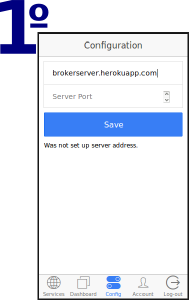
\includegraphics[width=7.5cm]{config.png}}
  \qquad
  \subfigure[fig:signup][Registro do usuário]{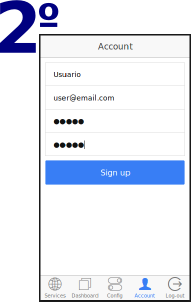
\includegraphics[width=7.5cm]{signup.png}}
\end{figure}
\begin{figure}[h]
  \qquad
  \subfigure[fig:log-in][Login na aplicação]{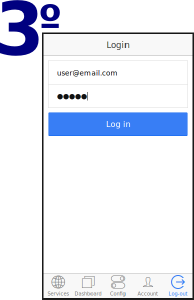
\includegraphics[width=7.5cm]{log-in.png}}
  \qquad
  \subfigure[fig:services][Listagem dos serviços]{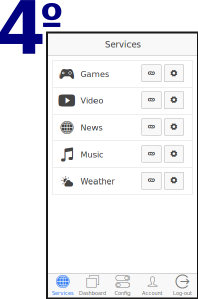
\includegraphics[width=7.5cm]{services.png}}
  \qquad
  \subfigure[fig:url][Cadastro das urls dos serviços]{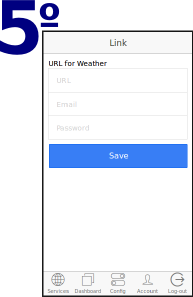
\includegraphics[width=7.5cm]{url.png}}
\end{figure}
\begin{figure}[h]
  \qquad
  \subfigure[fig:prefs][Configuração das preferências]{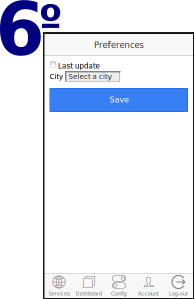
\includegraphics[width=7.5cm]{prefs.png}}
  \qquad
  \subfigure[fig:dash][Painel de apresentação do serviço]{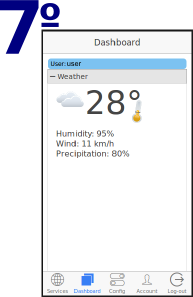
\includegraphics[width=7.5cm]{dash.png}}
\end{figure}
    %\anexo
    %\input{postextuais/anexo}
    \bibliographystyle{abnt-alf}
    \bibliography{tcc}
\end{document}